%%%%%%%%%%%%%%%%%%%%%%%%%%%%%%%%%%%%%%%%%%%%%%%%%%%
%% LaTeX book template                           %%
%% Author:  Amber Jain (http://amberj.devio.us/) %%
%% License: ISC license                          %%
%%%%%%%%%%%%%%%%%%%%%%%%%%%%%%%%%%%%%%%%%%%%%%%%%%%

\documentclass[a4paper,11pt]{report}
\usepackage[T1]{fontenc}
\usepackage[utf8]{inputenc}
\usepackage{lmodern}
\usepackage{tikz}
\usetikzlibrary{fadings}
\usetikzlibrary{patterns}
\usetikzlibrary{shadows.blur}
\usetikzlibrary{shapes}
\usepackage{indentfirst}
\usepackage{physics}
\usepackage{mathdots}
\usepackage{extarrows}
\usepackage{setspace}


%%%%%%%%%%%%%%%%%%%%%%%%%%%%%%%%%%%%%%%%%%%%%%%%%%%%%%%%%
% Source: http://en.wikibooks.org/wiki/LaTeX/Hyperlinks %
%%%%%%%%%%%%%%%%%%%%%%%%%%%%%%%%%%%%%%%%%%%%%%%%%%%%%%%%%
\usepackage{hyperref}
\usepackage{graphicx}
\usepackage[english]{babel}
\usepackage{fancyhdr}
\usepackage{mathtools}
\mathtoolsset{showonlyrefs} 

%%%%%%%%%%%%%%%%%%%%%%%%%%%%%%%%%%%%%%%%%%%%%%%%%%%%%%%%%%%%%%%%%%%%%%%%%%%%%%%%
% 'dedication' environment: To add a dedication paragraph at the start of book %
% Source: http://www.tug.org/pipermail/texhax/2010-June/015184.html            %
%%%%%%%%%%%%%%%%%%%%%%%%%%%%%%%%%%%%%%%%%%%%%%%%%%%%%%%%%%%%%%%%%%%%%%%%%%%%%%%%
\newenvironment{dedication}
{
   \cleardoublepage
   \thispagestyle{empty}
   \vspace*{\stretch{1}}
   \hfill\begin{minipage}[t]{0.66\textwidth}
   \raggedright
}
{
   \end{minipage}
   \vspace*{\stretch{3}}
   \clearpage
}

%% CODE STUFF
\usepackage{listings}
\usepackage{xcolor}

\definecolor{codegreen}{rgb}{0,0.6,0}
\definecolor{codegray}{rgb}{0.5,0.5,0.5}
\definecolor{codepurple}{rgb}{0.58,0,0.82}
\definecolor{backcolour}{rgb}{0.95,0.95,0.95}

\lstdefinestyle{mystyle}{
    backgroundcolor=\color{backcolour},   
    commentstyle=\color{codegreen},
    keywordstyle=\color{magenta},
    numberstyle=\tiny\color{codegray},
    stringstyle=\color{codepurple},
    basicstyle=\ttfamily\footnotesize,
    breakatwhitespace=false,         
    breaklines=true,                 
    captionpos=b,                    
    keepspaces=true,                 
    numbers=left,                    
    numbersep=5pt,                  
    showspaces=false,                
    showstringspaces=false,
    showtabs=false,                  
    tabsize=4
}

\setlength{\parskip}{12pt}

%%%%%%%%%%%%%%%%%%%%%%%%%%%%%%%%%%%%%%%%%%%%%%%%
% Chapter quote at the start of chapter        %
% Source: http://tex.stackexchange.com/a/53380 %
%%%%%%%%%%%%%%%%%%%%%%%%%%%%%%%%%%%%%%%%%%%%%%%%
\makeatletter
\renewcommand{\@chapapp}{}% Not necessary...
\newenvironment{chapquote}[2][2em]
  {\setlength{\@tempdima}{#1}%
   \def\chapquote@author{#2}%
   \parshape 1 \@tempdima \dimexpr\textwidth-2\@tempdima\relax%
   \itshape}
  {\par\normalfont\hfill--\ \chapquote@author\hspace*{\@tempdima}\par\bigskip}
\makeatother

%%%%%%%%%%%%%%%%%%%%%%%%%%%%%%%%%%%%%%%%%%%%%%%%%%%
% First page of book which contains 'stuff' like: %
%  - Book title, subtitle                         %
%  - Book author name                             %
%%%%%%%%%%%%%%%%%%%%%%%%%%%%%%%%%%%%%%%%%%%%%%%%%%%

% Book's title and subtitle
\title{\Huge \textbf{Flight Dynamics Bible}  \\ \huge Everything about 6 Degree of Freedom Modelling }
% Author
\author{\textsc{Hudson Reynolds}
\and
\textsc{Preston Wright}
}

\begin{document}

\pagestyle{fancy}
\renewcommand{\chaptermark}[1]{\markboth{#1}{#1}}
\fancyhead[R]{}
\fancyhead[L]{\thechapter\ --\ \leftmark}

\frontmatter
\maketitle

%%%%%%%%%%%%%%%%%%%%%%%%%%%%%%%%%%%%%%%%%%%%%%%%%%%%%%%%%%%%%%%
% Add a dedication paragraph to dedicate your book to someone %
%%%%%%%%%%%%%%%%%%%%%%%%%%%%%%%%%%%%%%%%%%%%%%%%%%%%%%%%%%%%%%%
% \begin{dedication}
% Dedicated to Calvin and Hobbes.
% \end{dedication}

%%%%%%%%%%%%%%%%%%%%%%%%%%%%%%%%%%%%%%%%%%%%%%%%%%%%%%%%%%%%%%%%%%%%%%%%
% Auto-generated table of contents, list of figures and list of tables %
%%%%%%%%%%%%%%%%%%%%%%%%%%%%%%%%%%%%%%%%%%%%%%%%%%%%%%%%%%%%%%%%%%

\begin{spacing}{.5}
    \tableofcontents
\end{spacing}
\
% \listoftables

\mainmatter

%%%%%%%%%%%
% Preface %
%%%%%%%%%%%



\chapter*{Preface}
Preston and I began working on the Flight Dynamics sub team in the fall of 2023. From May of 2024 to January 2025, we focused our efforts on creating a 6-DoF model from scratch. During this time, we learned a lot about the mathematics and physics involved in creating such a model. We were often faced with frustration in different conventions and poor explanations of certain topics, all of which were exacerbated by the difficulty of what we were learning. This made much of the material intractable. In this document, we hope to provide thorough explanations of all the necessary concepts in one place to make this journey easier for those who may need it in the future. 

Additionally, we hope this document can be used by those outside of the realm of flight dynamics to better understand the methodologies and inner workings of a 6-DoF model. Often, we have seen that a 6-DoF model is treated as a ‘black box’, where inputs go in and outputs come out. We hope that this document can provide a level of understanding adequate to allow greater collaboration between those working within and outside of flight dynamics.

In this document, we will be using excerpts of MATLAB script in some examples (code less than a page is included inline, and longer code is in the appendix) but our hope is that our explanations are thorough enough to facilitate the creation of a 6-DoF in any coding language. MATLAB facilitates the use of quite short code because of the number of built-in functions, but we include derivations for most of these equations or sources describing these derivations.

To use this document to its fullest extent, we recommend that you write scripts as you learn and use this document for reference and as a guide as you build or improve your own models.

In this first edition, we cover primarily the translational and rotational dynamics needed to set up a 6-DoF model. We also touch on subjects relating to the implementation of these equations in MATLAB and best practices. These are, in our opinion, the fundamental things that need to be understood before working on other aspects of a flight dynamics model. As such, these subjects comprise a large majority of both the effort and the length of the first edition.

Some other areas are also covered in this document but are not fully expounded because Preston and I have not the experience to give full authority on these subjects. However, as we learn more, this document is growing every day. In future editions, we hope to expand some of these other sections, especially relating to aerodynamics, to better serve those in the future who may hope to recreate the work we have done here.

% \section*{About the companion website}
% The website\footnote{\url{https://github.com/amberj/latex-book-template}} for this file contains:
% \begin{itemize}
%   \item A link to (freely downlodable) latest version of this document.
%   \item Link to download LaTeX source for this document.
%   \item Miscellaneous material (e.g. suggested readings etc).
% \end{itemize}

%%%%%%%%%%%%%%%%%%%%%%%%%%%%%%%%%%%%
% Give credit where credit is due. %
% Say thanks!                      %
%%%%%%%%%%%%%%%%%%%%%%%%%%%%%%%%%%%%
\section*{Acknowledgments}
\begin{itemize}
\item We would like give special thanks to Prof. Cunningham and Prof. Frueh for their help in reviewing our 6-DoF Model. Professor Frueh's notes have been especially helpful in compiling the information present in this document.

\end{itemize}

\chapter{Overview}

\begin{chapquote}{Carl Sagan}
``If you wish to make an apple pie from scratch, you must first invent the universe.''
\end{chapquote}

In much the same way, we must construct all of the mathematical background required to make a 6-DoF from the ground up. This chapter details the general requirements and an outline of the process we will be following.

\section{Necessary Background}
The goal of this document is to provide a comprehensive overview of the process and means to create, maintain, and build upon a 6 Degree of Freedom model. While we strive to make the document as easy as possible to understand, there are some instances where technical jargon is necessitated, and a strong understanding of mathematical concepts is required. 

Any time important technical jargon is required, we will \textit{italicize} the word for recognition. It is important to learn these terms to effectively and concisely describe your work. That being said, we attempt to keep the usage of jargon to a minimum. Because we italicize words in this manner, we choose to additionally underline any book titles present in the text.

To aid in comprehensibility, we have added sources that we find especially useful and avoided the use of superfluous sources. These sources are cited in the ISO 690 standard for ease of use to the reader. Additionally, useful links and footnotes have been highlighted in red boxes to be easily located.

To fully comprehend and successfully use this document, it is recommended that you have a good understanding of calculus, linear algebra, and calculus-based physics. A rudimentary understanding of differential equations and dynamics will also prove useful but is not strictly required.

Some concepts will arise in this document that are derived from graduate-level coursework and complex mathematics. In these instances, we may not attempt to derive the background and full understanding, but rather only what is necessary for building a 6-DoF model. In these cases, we also try to link to source material if you are inclined to learn more about those topics.

\section{Why 6-DoF?}
Let’s start off with some terminology in this section. A \textit{DoF} refers to a degree of freedom. In the language of flight dynamics, this refers to the number of ways an object can move in space. A more technically precise and rigorous definition defines this as the number of independent parameters that define the state. It is common to see 1-DoF, 3-DoF, and 6-DoF models all used in aerospace applications. Each of these are useful constructs, and often a simulation with more degrees of freedom is not necessarily better, depending on the scenario.

\subsection{1-DoF}
The first modeling that is often done for the sizing of rockets may use 1-DoF modeling. In this type of model, there is only one axis along which an object may translate or rotate about. In this case of rocket modeling, the only degree of freedom is the vertical height of the rocket. The goal of this type of model is mainly to provide a heuristic for determining rocket performance in the very preliminary stages of sizing by estimating the maximum altitude they can achieve.

Another example of this type of model is a simple mass-spring system along one axis. Such models may be useful for estimating the vibrations of bodies or as a first order approximation of fuel slosh.

We will use the example of a 1-DoF in section 2.1 to explain the creation of equations of motion in the simplest way. However, these models are often too constrained to give the most valuable information about a system, which is why 3-DoF and 6-DoF models are more often used.
\subsection{3-DoF}
After 1-DoF, the next step up is often a 3-DoF model. This type of model should be familiar to all flight dynamics members, as it is the subject of our onboarding project. In a 3-DoF model, there may be any combination of translational degrees of freedom and rotational degrees of freedom.

Often, 3-DoF modelling is utilized when either the rotational dynamics or translational dynamics of an object are considered unimportant. One example of this may be the calculation of an interplanetary transfer. The primary concern of the simulation is not the orientation of the satellite, but rather the location and velocity of the satellite at various points in 3D space. 

Another example of this type of model is planar motion. Often, problems in engineering are constrained in some way. Very often, we can consider one of the translational degrees of freedom to be non-important to the problem. This simplification allows us to greatly reduce the scope of the problem. One consequence of this action is that rotations are only permitted in a single axis. With two translational and one rotational degree of freedom, we can create useful models of many systems without great complexity.

Although the rest of this document will discuss 6-DoF models, really consider if you need that full complexity for your model! Often, a 3-DoF model is perfectly adequate for a large variety of problems without the hassle incurred by a 6-DoF model. 
\subsection{6-DoF}
6-DoF models are the most complex representation of a mechanical system. In 3D-space, there are only 6 possible degrees of freedom, and we simulate the dynamics in all of them.

Doing so is quite a difficult challenge, but it is not insurmountable. With careful planning, it is possible to gain an appreciation and understanding of the dynamics of a full 3D system. Doing so allows unrivaled modeling potential. In the case of a rocket, the primary reason that modeling in 6-DoF is so important is because it allows us to analyze the aerodynamic stability of the system. In both 1-DoF and 3-DoF modeling, this important aspect of the system is largely neglected.
\subsection{Structure Hierarchy of a 6-DoF}
An ideal 6-DoF not only models the motion of a vehicle through the atmosphere as accurately as possible but is also well-structured and easily readable. Strict adherence to an agreed upon and appropriate set of coding standards is essential for a successful program. These cover everything from naming conventions to heading structure, and make the integration of codes from multiple contributors more seamless.

Within the structure of a 6-DoF, there are three main, large “blocks” of code that are executed in sequence. The first is the initialization section. This is where all known, fixed parameters of the vehicle, atmosphere, and physics are initialized to be called later in the program. The second section is the integrator. This block utilizes a certain integration scheme to step through time, calculating the derivatives of the vehicle’s \textit{state vector}. Within the integrator, there are two major sub-blocks corresponding to two sets of dynamics: the forces and the moments. The forces section takes on the more familiar Newtonian Dynamics – regarding Position, Velocity, and Acceleration - that are seen in a high school physics class. The moments section takes on the Attitude Dynamics – orientation in space - of the vehicle. This can take the form of either Euler Angles or Parameters, which will be discussed further later. The final block is the visualizer block. This section writes pertinent information to matrices, animates the movement of the vehicle from launch to land, and outputs graphs of important metrics for the user to visualize.

Each of the previously mentioned sections will be discussed in more detail throughout this document.

\chapter{Newtonian Dynamics}
The first step when approaching any physics problem of this type is to consider the Newtonian dynamics of the system. In our case, we define Newtonian dynamics as only the translational dynamics of the system. You may often here this being referred to as particle dynamics. We will see later that attitude dynamics in 3D are more complicated, and for the sake of clarity will be explored separately from translational dynamics. 
\section{The 1-DoF Case:}
To begin our exploration of Newtonian dynamics, we will return to the example of the 1-DoF which we used earlier. Our goal with this is to use a simple example you are familiar with from high school physics and bring it up to speed with the terminology and techniques we will use for more complex analysis.

In Figure 1 below, we show an example of a very simple 1-DoF system free body diagram. We will use this example to explain the process of calculating the Newtonian dynamics in 1-dimension, which we then expand to the full 3D case. 

\tikzset{every picture/.style={line width=0.75pt}} %set default line width to 0.75pt        

\begin{figure}[h]
    \centering
    %\includegraphics[width=0.5\linewidth]{}
    
    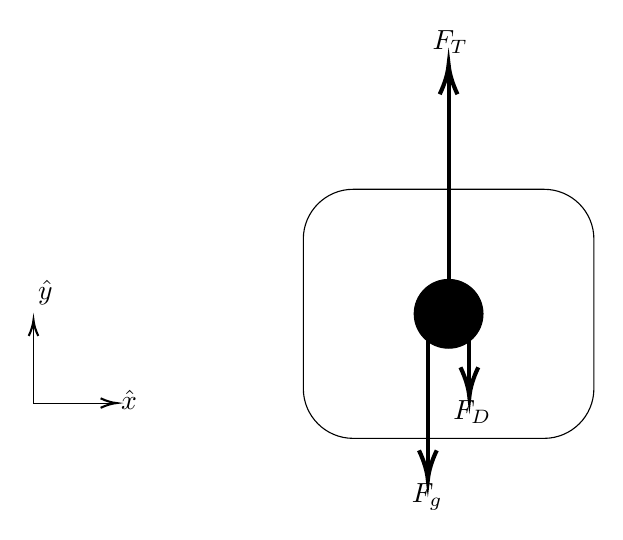
\begin{tikzpicture}[x=0.75pt,y=0.75pt,yscale=-1,xscale=1]
%uncomment if require: \path (0,308); %set diagram left start at 0, and has height of 308

%Rounded Rect [id:dp5842362308374554] 
\draw  [color={rgb, 255:red, 0; green, 0; blue, 0 }  ,draw opacity=1 ][fill={rgb, 255:red, 255; green, 255; blue, 255 }  ,fill opacity=1 ] (260,144) .. controls (260,130.75) and (270.75,120) .. (284,120) -- (376,120) .. controls (389.25,120) and (400,130.75) .. (400,144) -- (400,216) .. controls (400,229.25) and (389.25,240) .. (376,240) -- (284,240) .. controls (270.75,240) and (260,229.25) .. (260,216) -- cycle ;
%Straight Lines [id:da22630541270037763] 
\draw [line width=1.5]    (330,180) -- (330,63) ;
\draw [shift={(330,60)}, rotate = 90] [color={rgb, 255:red, 0; green, 0; blue, 0 }  ][line width=1.5]    (14.21,-4.28) .. controls (9.04,-1.82) and (4.3,-0.39) .. (0,0) .. controls (4.3,0.39) and (9.04,1.82) .. (14.21,4.28)   ;
%Straight Lines [id:da4912651471508729] 
\draw [line width=1.5]    (340,180) -- (340,217) ;
\draw [shift={(340,220)}, rotate = 270] [color={rgb, 255:red, 0; green, 0; blue, 0 }  ][line width=1.5]    (14.21,-4.28) .. controls (9.04,-1.82) and (4.3,-0.39) .. (0,0) .. controls (4.3,0.39) and (9.04,1.82) .. (14.21,4.28)   ;
%Shape: Circle [id:dp11471774870022611] 
\draw  [fill={rgb, 255:red, 0; green, 0; blue, 0 }  ,fill opacity=1 ] (313.44,180) .. controls (313.44,170.85) and (320.85,163.44) .. (330,163.44) .. controls (339.15,163.44) and (346.56,170.85) .. (346.56,180) .. controls (346.56,189.15) and (339.15,196.56) .. (330,196.56) .. controls (320.85,196.56) and (313.44,189.15) .. (313.44,180) -- cycle ;
%Straight Lines [id:da07105152032768414] 
\draw    (130,223) -- (130,185) ;
\draw [shift={(130,183)}, rotate = 90] [color={rgb, 255:red, 0; green, 0; blue, 0 }  ][line width=0.75]    (7.65,-2.3) .. controls (4.86,-0.97) and (2.31,-0.21) .. (0,0) .. controls (2.31,0.21) and (4.86,0.98) .. (7.65,2.3)   ;
%Straight Lines [id:da477096952774564] 
\draw    (130,223) -- (168,223) ;
\draw [shift={(170,223)}, rotate = 180] [color={rgb, 255:red, 0; green, 0; blue, 0 }  ][line width=0.75]    (7.65,-2.3) .. controls (4.86,-0.97) and (2.31,-0.21) .. (0,0) .. controls (2.31,0.21) and (4.86,0.98) .. (7.65,2.3)   ;
%Straight Lines [id:da5415789935745218] 
\draw [line width=1.5]    (320,180) -- (320,257) ;
\draw [shift={(320,260)}, rotate = 270] [color={rgb, 255:red, 0; green, 0; blue, 0 }  ][line width=1.5]    (14.21,-4.28) .. controls (9.04,-1.82) and (4.3,-0.39) .. (0,0) .. controls (4.3,0.39) and (9.04,1.82) .. (14.21,4.28)   ;

% Text Node
\draw (331,220.4) node [anchor=north west][inner sep=0.75pt]    {$F_{D}$};
% Text Node
\draw (321,42.4) node [anchor=north west][inner sep=0.75pt]    {$F_{T}$};
% Text Node
\draw (171,215.4) node [anchor=north west][inner sep=0.75pt]    {$\hat{x}$};
% Text Node
\draw (131,162.4) node [anchor=north west][inner sep=0.75pt]    {$\hat{y}$};
% Text Node
\draw (311,260.4) node [anchor=north west][inner sep=0.75pt]    {$F_{g}$};


\end{tikzpicture}
    \caption{1-DoF Forces on a body}
    \label{Figure 1}
\end{figure}

In Figure \ref{Figure 1}, a total of three forces are shown, all of which act along the  direction. The colinearity of all these forces is what makes this a 1-DoF model. The three forces shown are the thrust force, the drag force, and the gravity force.

Following what you may do in an introductory physics class, we will describe each of these forces via their functional form. These are described in Table \ref{Force Equations 1 DoF}. 

\begin{table}
\centering
\caption{Functional Form of Force Equations}
\label{Force Equations 1 DoF}
\begin{tabular}{l | l}
Force & Functional Form \\
\hline
 $F_g$&  $-mg$\\
 $F_D$&  $-1/2 \rho_{\infty} V^2_{\infty}SC_D$\\
 $F_T$&  $F_T\cdot[1-u(t-t_b)], t\le0$\\

\end{tabular}

\end{table}
The notation here is important to understand. In future AAE classes at Purdue, this is likely the notation that you will see. Terms with the subscript $\infty$ denote \textit{freestream} quantities, those that are freely flowing far away from the body of interest. Also of note is the unit step function, which is a function which has value zero until reaching time $t_b$, where it thereafter equals one. The quantity  $\rho$ refers to the density of the fluid, and $S$ to the \textit{reference area}. The \textit{drag coefficient} is $C_D$, a term which encapsulates the very complex nature of the fluid flow around an object. Calculating the value of  will be explored more deeply in later sections of this document. For now, we may assume a constant value.

It is helpful to think about these quantities as vectors, because we can add them together to achieve a resultant.\footnote{More formally, we define this as a linear space, where multiplicative and additive properties are preserved. This formal definition allows us to apply this to any arbitrarily number of dimensions. } In the 1-dimensional case this is quite trivial since all vectors along the  unit vector, but this will become increasingly important as we move to higher dimensions.
\subsection{Numerical Integration in the 1-DoF}
Now we will move into something that you may have not seen before. Given all the forces, we normally apply Newton’s 2\textsuperscript{nd} Law, $\sum{\vec{F}}=m\vec{a}$ , to arrive at an expression for the acceleration as shown in \eqref{eq2}. Doing so might look something like this:
\begin{gather}
F_T \cdot [1-u(t-t_b)]-\frac{1}{2}\rho_{\infty}V_{\infty}^2SC_D-mg=m\vec{a}\label{eq1} \\
\vec{a}=\frac{F_T \cdot [1-u(t-t_b)]-\frac{1}{2}\rho_{\infty}V_{\infty}^2SC_D}{m}-g\label{eq2}
\end{gather}
 From here, we use integration to find the velocity and then position of the object with time. Formally, we might define this formally as:
 $$\vec{V}=\int{\vec{a}}{dt}$$

However, you may notice something strange with our equation. In our expression for acceleration, we need to know the velocity. However, we do not know the velocity without integrating the equation first. This puts us in a chicken v. egg situation, so we must take a different approach to the problem. \footnote{Sometimes systems like this can be solved with traditional ODE methods. However, most complex systems like our 6-DoF have no known analytical solutions. We will focus on numerical integration because it will be more useful in general. }

The way we resolve this is to make an approximation of the solution in a process called \textit{Numerical Integration. }Here, we will outline the simplest type of numerical integration, known as Euler’s Method. This section aims to show how to implement Euler’s method in code, and the mathematical reasoning will be given a more formal treatment in section 5. We will describe more complex numerical integration schemes and why you might want to use them, but it’s good to see the code for a simple case first.

Euler’s Method involves discretizing our time interval. You may remember the concept of a Riemann Sum from calculus, where you approximate an integral in discrete time steps. We will take a similar approach with Euler’s Method. Euler’s method is applicable to solving first order ordinary differential equations (ODE’s). However, in our problem, we have a second order differential equation, because $\vec{a}=\ddot{y}$.

To resolve this issue, we will make this one differential equation into a system of first order differential equations. In general, we can convert an nth-order ODE into a system of n first-order ODEs.

In this case, we define a variable, . Now, we can express equation \eqref{eq2} as a system of two differential equations:

\begin{gather}\label{system}
        \dot{v}=\frac{F_T \cdot [1-u(t-t_b)]-\frac{1}{2}\rho_{\infty}V_{\infty}^2SC_D}{m}-g\\
    \dot{y}=v
\end{gather}

Now, we will apply Euler’s method to solve the problem. We will use the following steps to do so, using equation \eqref{system}as our example:

1. Rewrite the system in Leibniz notation, where $\dot{x}=\frac{dx}{dt}$.

2. Perform separation of variables, to arrive at $dx=v\cdot dt$.

3. Discretize the equation by ‘converting’  $dx$ and $dt$ to $\Delta x$ and $\Delta t$.\footnote{Note that we are not ‘converting’ in the sense of an equality, since the equations are no longer equivalent when we convert a differential element into a discrete one. We are just making an approximation of the true solution. Luckily, numerical integration schemes can get us quite close to true solutions. }

4. Rewrite $\Delta x$ as $x_{new}-x_{old}$. We can rearrange the equation as $x_{new}=v\cdot \Delta t + x_{old}$

5. To start, we define an initial state. This initial state will be the first value of $x_{old}$. 

6. Iterate through values of $\Delta t$ until the desired time of simulation is achieved.

We follow the same process for the integration of acceleration to find the velocity. Of note, we will use the previous value of $v$ in the computation of the new acceleration. Note that a more formal definition of Euler’s method is given in section 5.1.

We also show this example in MATLAB Script \ref{Script 1} below. Note that $\frac{1}{2}\rho_{\infty}SC_D$ is called $k$ in the script for simplicity. This simplification assumes that $\rho_{\infty}$ and the $C_D$ are constant, which we will later see is a quite poor assumption but is okay for a first approximation.

\lstset{style=mystyle}

\lstinputlisting[language=Matlab]{OneDofEuler.m}\label{Script 1}

There are a few important things to note about the MATLAB implementation of the script. Firstly, the only force that is defined outside of the loop is gravity, because the magnitude and direction of this force is independent of the current state of the system. We contrast this with the drag force and the thrust, which must be calculated on every iteration through the algorithm to find an updated value for the force.

We also note the use of the Heaviside function. This is functionally identical to a unit step function, just a different notation.

\section{The 3-DoF Case}
\subsection{Vectors in the 3-DoF Case:}
For Newtonian Dynamics, the most complex case is full 3D translational motion. Luckily, nothing very fundamental changes as compared to the 1-DoF case. The most important difference is the use of vector notation for compactness and clarity of mathematics and code. For position ($\vec{r}$), velocity ($\vec {v}$), and acceleration ($\vec{a}$), we represent them as tri-dimensional column vectors:

\begin{gather}
    \vec{r}=\begin{bmatrix}
        x_1\\
        x_2\\
        x_3
    \end{bmatrix},
    \vec{v}=\begin{bmatrix}
        \dot{x}_1\\
        \dot{x}_2\\
        \dot{x}_3\\
    \end{bmatrix},
        \vec{a}=\begin{bmatrix}
        \ddot{x}_1\\
        \ddot{x}_2\\
        \ddot{x}_3\\
    \end{bmatrix}
\end{gather}
This is done not only for the sake of compactness, but also to facilitate the use of matrix operations for translation between reference frames. This concept is further explored in section 3. For this reason, expressing these elements in vectors will become crucial as we move forward. In MATLAB, we express a tri-dimensional column vector as:
\begin{lstlisting}
pos=[0;0;0];
\end{lstlisting}
Where each semicolon represents a new row of the vector. We define a row vector by using a comma instead of a semicolon: 

\begin{lstlisting}
pos=[0,0,0];
\end{lstlisting}
Often, it is useful to convert between a row and column vector in MATLAB because some functions will expect the input to be in a different format. We can do so with a transposition. In MATLAB, this looks like: 

\begin{lstlisting}
pos=[0,0,0];
\end{lstlisting}

\subsection{Vector directions in the 3-DoF}
We present below a modified version of the 1-DoF below in full 3D in Figure \ref{fig:3 DoF Forces}.


\tikzset{every picture/.style={line width=0.75pt}} %set default line width to 0.75pt        

\begin{figure}[h]
    \centering
    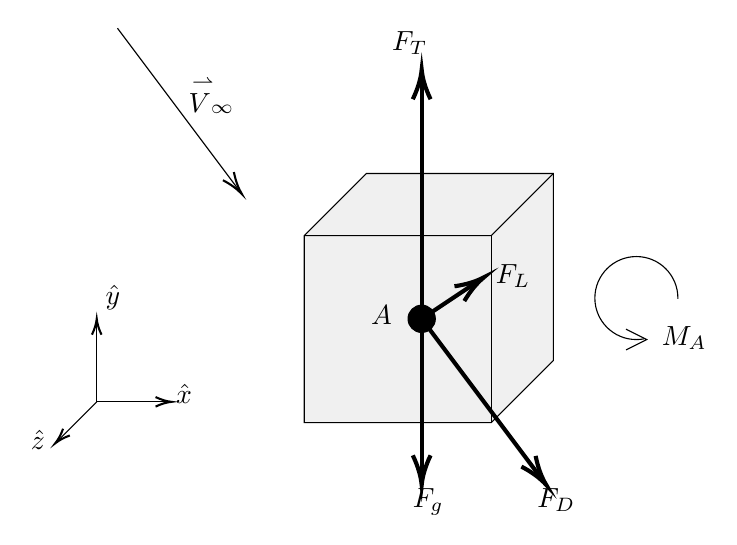
\begin{tikzpicture}[x=0.75pt,y=0.75pt,yscale=-1,xscale=1]
%uncomment if require: \path (0,308); %set diagram left start at 0, and has height of 308

%Shape: Cube [id:dp15885218660825062] 
\draw  [fill={rgb, 255:red, 155; green, 155; blue, 155 }  ,fill opacity=0.15 ] (260,129.92) -- (289.92,100) -- (380,100) -- (380,190.08) -- (350.08,220) -- (260,220) -- cycle ; \draw   (380,100) -- (350.08,129.92) -- (260,129.92) ; \draw   (350.08,129.92) -- (350.08,220) ;
%Straight Lines [id:da7537274804871096] 
\draw    (160,210) -- (160,172) ;
\draw [shift={(160,170)}, rotate = 90] [color={rgb, 255:red, 0; green, 0; blue, 0 }  ][line width=0.75]    (7.65,-2.3) .. controls (4.86,-0.97) and (2.31,-0.21) .. (0,0) .. controls (2.31,0.21) and (4.86,0.98) .. (7.65,2.3)   ;
%Straight Lines [id:da28051238395124845] 
\draw    (160,210) -- (194,210) ;
\draw [shift={(196,210)}, rotate = 180] [color={rgb, 255:red, 0; green, 0; blue, 0 }  ][line width=0.75]    (7.65,-2.3) .. controls (4.86,-0.97) and (2.31,-0.21) .. (0,0) .. controls (2.31,0.21) and (4.86,0.98) .. (7.65,2.3)   ;
%Straight Lines [id:da0491508391303197] 
\draw    (160,210) -- (141.41,228.59) ;
\draw [shift={(140,230)}, rotate = 315] [color={rgb, 255:red, 0; green, 0; blue, 0 }  ][line width=0.75]    (7.65,-2.3) .. controls (4.86,-0.97) and (2.31,-0.21) .. (0,0) .. controls (2.31,0.21) and (4.86,0.98) .. (7.65,2.3)   ;
%Straight Lines [id:da4424478744689285] 
\draw    (170,30) -- (228.8,108.4) ;
\draw [shift={(230,110)}, rotate = 233.13] [color={rgb, 255:red, 0; green, 0; blue, 0 }  ][line width=0.75]    (10.93,-3.29) .. controls (6.95,-1.4) and (3.31,-0.3) .. (0,0) .. controls (3.31,0.3) and (6.95,1.4) .. (10.93,3.29)   ;
%Straight Lines [id:da9341165159771404] 
\draw [line width=1.5]    (316.56,170) -- (316.56,247) ;
\draw [shift={(316.56,250)}, rotate = 270] [color={rgb, 255:red, 0; green, 0; blue, 0 }  ][line width=1.5]    (14.21,-4.28) .. controls (9.04,-1.82) and (4.3,-0.39) .. (0,0) .. controls (4.3,0.39) and (9.04,1.82) .. (14.21,4.28)   ;
%Straight Lines [id:da4700324062294746] 
\draw [line width=1.5]    (316.56,170) -- (374.76,247.6) ;
\draw [shift={(376.56,250)}, rotate = 233.13] [color={rgb, 255:red, 0; green, 0; blue, 0 }  ][line width=1.5]    (14.21,-4.28) .. controls (9.04,-1.82) and (4.3,-0.39) .. (0,0) .. controls (4.3,0.39) and (9.04,1.82) .. (14.21,4.28)   ;
%Straight Lines [id:da6206056974950449] 
\draw [line width=1.5]    (316.56,170) -- (316.56,53) ;
\draw [shift={(316.56,50)}, rotate = 90] [color={rgb, 255:red, 0; green, 0; blue, 0 }  ][line width=1.5]    (14.21,-4.28) .. controls (9.04,-1.82) and (4.3,-0.39) .. (0,0) .. controls (4.3,0.39) and (9.04,1.82) .. (14.21,4.28)   ;
%Shape: Circle [id:dp9278618893074794] 
\draw  [fill={rgb, 255:red, 0; green, 0; blue, 0 }  ,fill opacity=1 ] (310,170) .. controls (310,166.38) and (312.94,163.44) .. (316.56,163.44) .. controls (320.19,163.44) and (323.13,166.38) .. (323.13,170) .. controls (323.13,173.62) and (320.19,176.56) .. (316.56,176.56) .. controls (312.94,176.56) and (310,173.62) .. (310,170) -- cycle ;
%Straight Lines [id:da05847350311292765] 
\draw [line width=1.5]    (316.56,170) -- (344.07,151.66) ;
\draw [shift={(346.56,150)}, rotate = 146.31] [color={rgb, 255:red, 0; green, 0; blue, 0 }  ][line width=1.5]    (14.21,-4.28) .. controls (9.04,-1.82) and (4.3,-0.39) .. (0,0) .. controls (4.3,0.39) and (9.04,1.82) .. (14.21,4.28)   ;
%Shape: Arc [id:dp5580370574812169] 
\draw  [draw opacity=0] (423.67,179.66) .. controls (422.48,179.88) and (421.25,180) .. (420,180) .. controls (408.95,180) and (400,171.05) .. (400,160) .. controls (400,148.95) and (408.95,140) .. (420,140) .. controls (431.05,140) and (440,148.95) .. (440,160) .. controls (440,160.15) and (440,160.29) .. (440,160.44) -- (420,160) -- cycle ; \draw   (423.67,179.66) .. controls (422.48,179.88) and (421.25,180) .. (420,180) .. controls (408.95,180) and (400,171.05) .. (400,160) .. controls (400,148.95) and (408.95,140) .. (420,140) .. controls (431.05,140) and (440,148.95) .. (440,160) .. controls (440,160.15) and (440,160.29) .. (440,160.44) ;  
\draw   (415,175) -- (425,180) -- (415,185) ;

% Text Node
\draw (197,200.4) node [anchor=north west][inner sep=0.75pt]    {$\hat{x}$};
% Text Node
\draw (163,152.4) node [anchor=north west][inner sep=0.75pt]    {$\hat{y}$};
% Text Node
\draw (127,222.4) node [anchor=north west][inner sep=0.75pt]    {$\hat{z}$};
% Text Node
\draw (203,52.4) node [anchor=north west][inner sep=0.75pt]    {$\stackrel {\rightharpoonup}{V}_{\infty }$};
% Text Node
\draw (311,250.4) node [anchor=north west][inner sep=0.75pt]    {$F_{g}$};
% Text Node
\draw (371,250.4) node [anchor=north west][inner sep=0.75pt]    {$F_{D}$};
% Text Node
\draw (301,30.4) node [anchor=north west][inner sep=0.75pt]    {$F_{T}$};
% Text Node
\draw (351,142.4) node [anchor=north west][inner sep=0.75pt]    {$F_{L}$};
% Text Node
\draw (431,172.4) node [anchor=north west][inner sep=0.75pt]    {$M_{A}$};
% Text Node
\draw (291,162.4) node [anchor=north west][inner sep=0.75pt]    {$A$};


\end{tikzpicture}

    \caption{3-DoF Forces on a Body}
    \label{fig:3 DoF Forces}
\end{figure}



As compared to 1-DoF case, we have three new quantities that are present. The first of these is $\vec{V}_{\infty}$, the freestream airflow vector, being shown on the diagram.\footnote{Freestream velocity  is drawn in the direction of incoming air by convention. However, for calculations, we will use the convention that  is the direction of the velocity of the vehicle (opposite sign to drawing).} This is represented diagrammatically because it no longer must be along the $\hat{y}$ direction. When we have an angle between the nose (the direction through which the thrust force points in Figure 2) and the freestream velocity, we refer to this as an \textit{angle of attack}. This angle of attack is often denoted with the letter $\alpha$. We will discuss angle of attack and its effects more in section 4. For now, we simply need to understand how to calculate  given the vector through the nose and the freestream velocity vector.

To do this, we use the fact that the dot product is related to the cosine of the angle between the vectors. Denoting the vector through the nose of the rocket , we can find the angle of attack as:
\begin{equation}\label{eq:alpha}
    \alpha=cos^{-1}\left(\frac{\hat{X}\cdot \vec{V}_{\infty}}{||\hat{X}||\ ||\vec{V}_{\infty}||}\right)
\end{equation}

The next new quantity is $F_L$, the force of lift. The force of lift is always perpendicular in direction to $\vec{V}_{\infty}$. Knowing this, we can find the direction of the force of lift as:
\begin{equation}\label{eq:Lift}
    \hat{L}=\frac{(\hat{V}_{\infty} \times \hat{X}) \times \hat{V}_{\infty}}{||(\hat{V}_{\infty} \times \hat{X}) \times \hat{V}_{\infty}||}
\end{equation}
Here, the cross product is used because it generates a vector orthogonal to the two input vectors. This is exactly the property that we need when defining lift.

For the sake of completeness, we should also note that the force of drag lies opposite the direction of . This is much simpler to calculate, and looks like:
$$\hat{D}=\frac{-\hat{V}_{\infty}}{||\hat{V}_{\infty}||}$$

The last force directions to define are the direction of thrust and the direction of gravity. Luckily, these are easily defined because they point directly along basis vectors.\footnote{We assume here that there is no misalignment in the thrust vector and it is coincident with the  vector.} The force of gravity is defined with respect to the inertial reference frame and is defined in \eqref{eq:Fg}. The force of thrust is defined with respect to the vector pointing through the nose, $\hat{X}$, and is shown in \eqref{eq:Ft}:
\begin{equation}\label{eq:Fg}
    \vec{F}_g=-mg\cdot \hat{y}
\end{equation}
\begin{equation}\label{eq:Ft}
    \vec{F}_T=F_T\cdot \hat{X}
\end{equation}
\subsection{Moments}
The last new quantity is the moment about point A, denoted $M_A$. For now, we will simply note that for an arbitrary selection of point A, we will have a rotational moment that is generated because the forces on the body do not necessarily act through point A, even if it is the center of mass (see section 4 for more details). In Figure\ref{fig:3 DoF Forces}, we have drawn all of the forces acting through a single point for simplicity, but this is not generally the case.

For our rocket modeling, it is generally assumed that gravity and thrust act about the center of gravity, and the aerodynamic forces about the center of pressure (more on this in 4.1.1).

We will show how to compute this moment if the location of the center of gravity and the center of pressure is known. To show this, we will briefly return the 2D case for illustration, but keep in mind that this concept is extensible in 3D. We show this in Figure \ref{fig:Moments}.

\begin{figure}
    \centering
    
\tikzset{every picture/.style={line width=0.75pt}} %set default line width to 0.75pt        

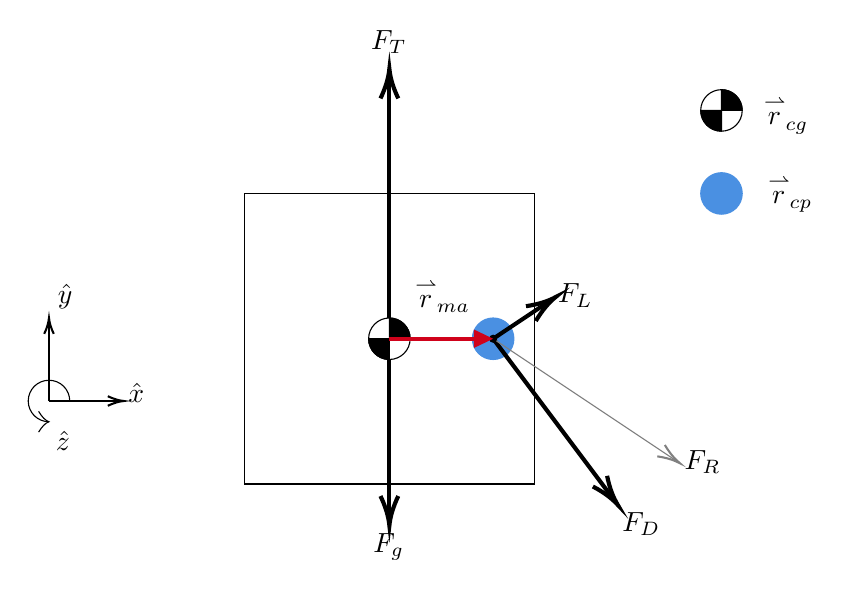
\begin{tikzpicture}[x=0.75pt,y=0.75pt,yscale=-1,xscale=1]
%uncomment if require: \path (0,300); %set diagram left start at 0, and has height of 300

%Shape: Rectangle [id:dp16059631350753278] 
\draw   (224,90) -- (364,90) -- (364,230) -- (224,230) -- cycle ;
%Shape: Circle [id:dp26152316559967836] 
\draw   (284,160) .. controls (284,154.48) and (288.48,150) .. (294,150) .. controls (299.52,150) and (304,154.48) .. (304,160) .. controls (304,165.52) and (299.52,170) .. (294,170) .. controls (288.48,170) and (284,165.52) .. (284,160) -- cycle ;
%Straight Lines [id:da4396178512453982] 
\draw [line width=1.5]    (294,150) -- (294,33) ;
\draw [shift={(294,30)}, rotate = 90] [color={rgb, 255:red, 0; green, 0; blue, 0 }  ][line width=1.5]    (14.21,-4.28) .. controls (9.04,-1.82) and (4.3,-0.39) .. (0,0) .. controls (4.3,0.39) and (9.04,1.82) .. (14.21,4.28)   ;
%Straight Lines [id:da6367078669315451] 
\draw [line width=1.5]    (294,170) -- (294,247) ;
\draw [shift={(294,250)}, rotate = 270] [color={rgb, 255:red, 0; green, 0; blue, 0 }  ][line width=1.5]    (14.21,-4.28) .. controls (9.04,-1.82) and (4.3,-0.39) .. (0,0) .. controls (4.3,0.39) and (9.04,1.82) .. (14.21,4.28)   ;
%Shape: Circle [id:dp9868324677149697] 
\draw  [color={rgb, 255:red, 74; green, 144; blue, 226 }  ,draw opacity=1 ][fill={rgb, 255:red, 74; green, 144; blue, 226 }  ,fill opacity=1 ] (334,160) .. controls (334,154.48) and (338.48,150) .. (344,150) .. controls (349.52,150) and (354,154.48) .. (354,160) .. controls (354,165.52) and (349.52,170) .. (344,170) .. controls (338.48,170) and (334,165.52) .. (334,160) -- cycle ;
%Straight Lines [id:da08375154983020605] 
\draw [line width=1.5]    (344,160) -- (371.5,141.66) ;
\draw [shift={(374,140)}, rotate = 146.31] [color={rgb, 255:red, 0; green, 0; blue, 0 }  ][line width=1.5]    (14.21,-4.28) .. controls (9.04,-1.82) and (4.3,-0.39) .. (0,0) .. controls (4.3,0.39) and (9.04,1.82) .. (14.21,4.28)   ;
%Straight Lines [id:da9997269035553926] 
\draw [line width=1.5]    (344,160) -- (402.2,237.6) ;
\draw [shift={(404,240)}, rotate = 233.13] [color={rgb, 255:red, 0; green, 0; blue, 0 }  ][line width=1.5]    (14.21,-4.28) .. controls (9.04,-1.82) and (4.3,-0.39) .. (0,0) .. controls (4.3,0.39) and (9.04,1.82) .. (14.21,4.28)   ;
%Straight Lines [id:da3915949331033487] 
\draw [color={rgb, 255:red, 128; green, 128; blue, 128 }  ,draw opacity=1 ]   (344,160) -- (432.34,218.89) ;
\draw [shift={(434,220)}, rotate = 213.69] [color={rgb, 255:red, 128; green, 128; blue, 128 }  ,draw opacity=1 ][line width=0.75]    (10.93,-3.29) .. controls (6.95,-1.4) and (3.31,-0.3) .. (0,0) .. controls (3.31,0.3) and (6.95,1.4) .. (10.93,3.29)   ;
%Shape: Circle [id:dp6233406826761347] 
\draw  [fill={rgb, 255:red, 0; green, 0; blue, 0 }  ,fill opacity=1 ] (342.33,160) .. controls (342.33,159.08) and (343.08,158.33) .. (344,158.33) .. controls (344.92,158.33) and (345.67,159.08) .. (345.67,160) .. controls (345.67,160.92) and (344.92,161.67) .. (344,161.67) .. controls (343.08,161.67) and (342.33,160.92) .. (342.33,160) -- cycle ;
%Shape: Pie [id:dp5263153723129019] 
\draw  [fill={rgb, 255:red, 0; green, 0; blue, 0 }  ,fill opacity=1 ] (294,150) .. controls (294,150) and (294,150) .. (294,150) .. controls (299.52,150) and (304,154.48) .. (304,160) -- (294,160) -- cycle ;
%Shape: Pie [id:dp03519524739615432] 
\draw  [fill={rgb, 255:red, 0; green, 0; blue, 0 }  ,fill opacity=1 ] (294,170) .. controls (294,170) and (294,170) .. (294,170) .. controls (294,170) and (294,170) .. (294,170) .. controls (288.48,170) and (284,165.52) .. (284,160) -- (294,160) -- cycle ;
%Straight Lines [id:da5638933773253405] 
\draw [color={rgb, 255:red, 208; green, 2; blue, 27 }  ,draw opacity=1 ][line width=1.5]    (294,160) -- (340,160) ;
\draw [shift={(344,160)}, rotate = 180] [fill={rgb, 255:red, 208; green, 2; blue, 27 }  ,fill opacity=1 ][line width=0.08]  [draw opacity=0] (9.29,-4.46) -- (0,0) -- (9.29,4.46) -- cycle    ;
%Shape: Circle [id:dp854204209250383] 
\draw   (444,50) .. controls (444,44.48) and (448.48,40) .. (454,40) .. controls (459.52,40) and (464,44.48) .. (464,50) .. controls (464,55.52) and (459.52,60) .. (454,60) .. controls (448.48,60) and (444,55.52) .. (444,50) -- cycle ;
%Shape: Pie [id:dp5370740069872785] 
\draw  [fill={rgb, 255:red, 0; green, 0; blue, 0 }  ,fill opacity=1 ] (454,60) .. controls (454,60) and (454,60) .. (454,60) .. controls (454,60) and (454,60) .. (454,60) .. controls (448.48,60) and (444,55.52) .. (444,50) -- (454,50) -- cycle ;
%Shape: Pie [id:dp7640770799900009] 
\draw  [fill={rgb, 255:red, 0; green, 0; blue, 0 }  ,fill opacity=1 ] (454,40) .. controls (454,40) and (454,40) .. (454,40) .. controls (459.52,40) and (464,44.48) .. (464,50) -- (454,50) -- cycle ;
%Shape: Circle [id:dp281241699306923] 
\draw  [color={rgb, 255:red, 74; green, 144; blue, 226 }  ,draw opacity=1 ][fill={rgb, 255:red, 74; green, 144; blue, 226 }  ,fill opacity=1 ] (444,90) .. controls (444,84.48) and (448.48,80) .. (454,80) .. controls (459.52,80) and (464,84.48) .. (464,90) .. controls (464,95.52) and (459.52,100) .. (454,100) .. controls (448.48,100) and (444,95.52) .. (444,90) -- cycle ;
%Straight Lines [id:da2704614420307284] 
\draw    (130,190) -- (130,152) ;
\draw [shift={(130,150)}, rotate = 90] [color={rgb, 255:red, 0; green, 0; blue, 0 }  ][line width=0.75]    (7.65,-2.3) .. controls (4.86,-0.97) and (2.31,-0.21) .. (0,0) .. controls (2.31,0.21) and (4.86,0.98) .. (7.65,2.3)   ;
%Straight Lines [id:da24091737468013485] 
\draw    (130,190) -- (164,190) ;
\draw [shift={(166,190)}, rotate = 180] [color={rgb, 255:red, 0; green, 0; blue, 0 }  ][line width=0.75]    (7.65,-2.3) .. controls (4.86,-0.97) and (2.31,-0.21) .. (0,0) .. controls (2.31,0.21) and (4.86,0.98) .. (7.65,2.3)   ;
%Shape: Arc [id:dp6249807559731687] 
\draw  [draw opacity=0] (130,200) .. controls (130,200) and (130,200) .. (130,200) .. controls (130,200) and (130,200) .. (130,200) .. controls (124.48,200) and (120,195.52) .. (120,190) .. controls (120,184.48) and (124.48,180) .. (130,180) .. controls (135.52,180) and (140,184.48) .. (140,190) -- (130,190) -- cycle ; \draw   (130,200) .. controls (130,200) and (130,200) .. (130,200) .. controls (130,200) and (130,200) .. (130,200) .. controls (124.48,200) and (120,195.52) .. (120,190) .. controls (120,184.48) and (124.48,180) .. (130,180) .. controls (135.52,180) and (140,184.48) .. (140,190) ;  
\draw   (125,195) .. controls (126.67,197.78) and (128.33,199.44) .. (130,200) .. controls (128.33,200.56) and (126.67,202.22) .. (125,205) ;

% Text Node
\draw (284,10.4) node [anchor=north west][inner sep=0.75pt]    {$F_{T}$};
% Text Node
\draw (285,252.4) node [anchor=north west][inner sep=0.75pt]    {$F_{g}$};
% Text Node
\draw (374,132.4) node [anchor=north west][inner sep=0.75pt]    {$F_{L}$};
% Text Node
\draw (405,242.4) node [anchor=north west][inner sep=0.75pt]    {$F_{D}$};
% Text Node
\draw (435,212.4) node [anchor=north west][inner sep=0.75pt]    {$F_{R}$};
% Text Node
\draw (305,130.4) node [anchor=north west][inner sep=0.75pt]    {$\stackrel {\rightharpoonup}{r}_{ma}$};
% Text Node
\draw (473,42.4) node [anchor=north west][inner sep=0.75pt]    {$\stackrel {\rightharpoonup}{r}_{cg}$};
% Text Node
\draw (475,80.4) node [anchor=north west][inner sep=0.75pt]    {$\stackrel {\rightharpoonup}{r}_{cp}$};
% Text Node
\draw (167,180.4) node [anchor=north west][inner sep=0.75pt]    {$\hat{x}$};
% Text Node
\draw (133,132.4) node [anchor=north west][inner sep=0.75pt]    {$\hat{y}$};
% Text Node
\draw (132,203.4) node [anchor=north west][inner sep=0.75pt]    {$\hat{z}$};


\end{tikzpicture}

    \caption{Moment Demonstration}
    \label{fig:Moments}
\end{figure}
In Figure \ref{fig:Moments} we include a few new symbols. All force magnitudes, however, are equivalent to what we show in Figure 2 (with the assumption that they lie in the x-y plane for this example). We denote the location of the center of gravity as $\vec{r}_{cg}$ and the location of the center of pressure as $\vec{r}_{cp}$. The difference between $\vec{r}_{cg}$ and $\vec{r}_{cp}$ is denoted as $\vec{r}_{ma}$. We refer to this as the moment arm of the aerodynamic forces. It should be noted that all of locations are tridimensional vectors. 

We also define a new vector, $F_R$, the resultant aerodynamic vector, which is the vector sum of $F_D$ and $F_L$. Because free rotations occur about the center of mass, it is most helpful to calculate our final moment from this location. To do so, we use the moment equation:
$$M=\vec{r}\times \vec{F}_R$$
We note that the direction of this moment is in the $-\hat{z}$ direction due to the nature of the cross product.

One thing to note is that some quantities are more easily defined with respect to vectors that are defined with respect to the vehicle (which we will call the \textit{body frame}), such as the vector $\hat{X}$. As seen in \eqref{eq:alpha} and \eqref{eq:Lift}, we often want to use these vectors in the body frame for computation. As such, we will need a method in which we can convert between the body and inertial frames. This conversion between frames is explored in section \ref{sec:attitude dynamics}.
\subsection{}

\chapter{Attitude Dynamics}\label{sec:attitude dynamics}
\begin{chapquote}{Lord Kelvin, 1892}
``Quaternions came from Hamilton after his really good work had been done; and, though beautifully ingenious, have been an unmixed evil to those who have touched them in any way, including Clerk Maxwell.''
\end{chapquote}
\section{Frame of Reference}
\section{2-D Rotations}
\section{Euler Angles}
\section{Quaternions}
It was a gorgeous October day in Dublin, and William Hamilton was on a stroll with his wife on his way to the Royal Irish Academy. Having worked on Quaternions for some time, answers had been slowly forming in his head. As he crossed a cobblestone bridge above the Royal Canal, the answer of a necessary, fourth dimension for calculating triples struck him like a freight train. He hastily carved the fundamental formula for quaternion multiplication, $i^2+j^2+k^2=ijk=-1$, into the stones he was walking on. And so, \textit{quaternions} were born.


\chapter{Aerodynamic Modeling}
In section 2.2 we discussed the 4 fundamental forces on a vehicle and how we define their directions. In that section we did not define the magnitude of the aerodynamic forces, $F_L$ and $F_D$. The magnitude of these forces are quite difficult to calculate and require the most approximation to do correctly. The governing equation for calculating the magnitude of our aerodynamics is $\frac{1}{2}\rho_{\infty}V^2_{\infty}SC_X$, where $C_X$ is either $C_L$ or $C_D$.

Despite the innocuous appearance of this equation, calculating the aerodynamics of our system is deceptively hard because the calculation of  is very complicated. In fact, without real data, any calculation that we made of these values will just be an approximation.\footnote{Even with wind tunnel data, it is still likely that some approximations need to be made. Aerodynamics in general has no definite answers.} That being said, there are approaches we can take which will get us close enough to true values to prove useful.

Aerodynamics has a lot of terminology associated with it that is important to understand before we can approach modelling the aerodynamics of the system. We will mostly cover aerodynamics terminology for rockets, but the modelling done here should be transferable to aspects of aircraft systems as well.\footnote{The principles we describe are the same, but much of the modelling is simpler for rockets since they have axial symmetry in most cases. We will utilize these assumptions early on to simplify this section.}

When modelling aerodynamic forces, we can imagine that two differential force elements act at each point along the body. At each point, there is a pressure which acts normal to the surface and a shear stress (you can think of it as a friction) that acts tangentially to the surface. These are shown in Figure \ref{fig:pressure and shear}.

\begin{figure}
    \centering
    \includegraphics[width=\linewidth]{Images/ShearStress.png}
    \caption{Pressure and Shear Stress on an Aerodynamic Surface}
    \label{fig:pressure and shear}
\end{figure}


\section{Aerodynamics Terminology and Basics}
\section{Atmospheric Modelling}

\chapter{Numerical Integration Schemes}
For more information and derivations about the following section, refer to (3). This source includes some more information than included here and some useful examples.

\section{Euler Integration}
We have previously discussed the simplest integration scheme, the explicit Euler method, which we used in section 2.1.1. Understanding the Euler method is key to understanding and using more complex integration schemes, so we recommend writing a few of your own Euler integration scripts in MATLAB or a coding language of your choice to really solidify your knowledge before moving on to more complex integration schemes. 

We formalize the explicit Euler integration below. Given a linear ODE:

\section{Improved Euler / RK2}
Given the limitations of the Explicit Euler method, we will start by investigating the improved Euler Method. This improved Euler method is the first of a family of integration schemes known as Runge-Kutta (RK) integration schemes. The number, 2, represents the order of the integration scheme, which we will explore more later.

The main area that led to inaccuracies in the explicit Euler method was the slope that we calculated. We can improve on this by taking two points and finding the average slope. We choose to take a point at our start and our end point,  and , and evaluate the slope at both of those points and average them. From the previous section, we can remember that:
\begin{equation}
    y'=f\left(x_i,y(x_i)\right)
\end{equation}
So, we can write the average slope as
\begin{equation}
    m=\frac{y_1'+y_2'}{2}
\end{equation}
Where

\begin{gather}
    y_1'=f\left(x_i,y(x_i)\right)\\
    y_2'=f\left(x_{i+1},y(x_{i+1})\right)
\end{gather}
Now that we have the slope, we follow the same process as we did for the Explicit Euler method to find the next value. We take the slope and multiply it by the timestep, $\Delta t$, and add the current value, $y(x_i)$. This gives us our approximation as:
\begin{equation}
    y=y(x_i)+\frac{y_1'+y_2'}{2}\Delta t
\end{equation}
We can write this then as:
\begin{equation}
    y_{i+1}=y_i+\frac{\Delta t}{2}\left[f(x_i,y(x_i))+f(x_{i+1},y(x_{i+1}))\right]
\end{equation}
To rewrite this equation in a way that is better suited for code:
\begin{gather}\label{eq:rk2}
    k_1=f(x_i,y_i)\\\\
    k_2=f(x+\Delta t, y_i+\Delta tk_1)\\\\
    y_{i+1}=y_i+\frac{\Delta t}{2}(k_1+k_2)
\end{gather}
We can note here that this method requires at least two evaluations since $k_2$ is dependent on $k_1$. However, this is often still more computationally efficient than the Explicit Euler method because larger time steps can be used with lesser error.

\subsection{RK2 in Code}
Implementing the RK2 algorithm in code is slightly more complicated than implementing the explicit Euler method. To properly implement this, we will use \textit{function handles} in MATLAB. Function handles act as pointers to an instance of a function. To explain what that means, we will examine the following code snippet:

\begin{lstlisting}[language=Matlab]
f = @computeSquare;
a = 4;
b = f(a)
\end{lstlisting}
where 'computeSquare' is defined as:

\lstset{style=mystyle}
\begin{lstlisting}[language=Matlab]
function y = computeSquare(x)
y = x.\^2;
end
\end{lstlisting}

The function handle allows us to assign the function to a variable, which we are calling ‘f’\textit{.} We call this a pointer because this variable ‘points’ to the function ‘computeSquare’. 

In this example, when we call this operation, the value of b is 16.

A useful feature of function handles for numerical integration is that they allow us to pass in only the variables needed for numerical integration and pass other variables in the expression as constants. In general, we want our numerical scheme to only accept our state vector and the time vector. This is the same thing that ode45 does, so it is best practice to do the same thing here.

\section{RK4 Integration}
RK4 integration is the last major integration scheme that we will explore. RK4 integration is often the best balance between the precision of the algorithm and the speed of computation. 

To explain the RK4, we will go back to the RK2 and explain it in a slightly different way that will shed light on what we are doing with RK4. In RK2, we described taking the average slope of the function. We can also imagine taking the Taylor expansion of our function:
$$y_{i+1}=y_i+y_i'\Delta t+y_i''\frac{\Delta t}{2}+O\left(\Delta t^3\right)$$
From this Taylor expansion of the solution, we can that our approximation accounts for linear and quadratic terms. Thus, our error is proportional to terms to the 3\textsuperscript{rd} power, represented by $O(\Delta t^3)$. We know  and , but the 2\textsuperscript{nd }order derivative of our function is unknown. We can approximate this 2\textsuperscript{nd} order derivative as:
$$y_i=\frac{y'_{i+1}-y_i'}{\Delta t}$$
Upon rearranging this equation, we can see that we arrive at the same expression as we did before. We can apply the same approach for the RK4 integration, except we consider terms up to the 4\textsuperscript{th} order expansion of the Taylor series:
$$y_{i+1}=y_i+y_i'\Delta t+y_i''\frac{\Delta t}{2}+y_i'''\frac{\Delta t}{6}+y_i''''\frac{\Delta t}{24}O\left(\Delta t^5\right)$$
Immediately, we can see that our error has shrunk to be proportional to terms of the 5\textsuperscript{th} order, a dramatic reduction as compared to RK2 or Explicit Euler method.

\subsection{RK4 Integration in Code}
The RK4 Integration scheme can be expressed as a set of equations very similar to what we did with \eqref{eq:rk2}. We will not derive these equations here, because the process is very similar to that used for the RK2 method.

The form of these equations is shown in \eqref{eq:RK4}.
\begin{gather}\label{eq:RK4}
    y_{i+1}=y_i+\frac{\Delta t}{6}\left(k_1+2k_2+2k_3+k_4\right)\\\\
    k_1=f(x_i,y_i)\\
    k_2=\left(x_i+\frac{\Delta t}{2},y_i+\frac{\Delta t}{2}k_1\right)\\
    k_3=\left(x_i+\frac{\Delta t}{2},y_i+\frac{\Delta t}{2}k_2\right)\\
    k_4=f(x_i+\Delta t,y_i+\Delta tk_3)
\end{gather}
An implementation of this algorithm into code is shown below.
\begin{lstlisting}[language=Matlab]
    %% RK4 Integrator
% numerically integrates a first order initial value problem
% inputs:
% fun - function of integration
% dt - time step [s]
% tIn - input time [s]
% xIn - initial value input vector
% outputs:
% out - final value output vector
function out = rk4(fun, dt, tIn, xIn)
    f1 = fun(tIn,xIn);
    f2 = fun(tIn + dt/2, xIn + (dt/2) .* f1);
    f3 = fun(tIn + dt/2, xIn + (dt/2) .* f2);
    f4 = fun(tIn + dt, xIn + dt*f3);
    
    out = xIn + (dt / 6)*(f1 + 2*f2 + 2*f3+f4);
end
\end{lstlisting}

Often, we use a function in MATLAB called ode45 to perform RK4 integration. This function has the benefit that it will change the step size to produce high accuracy when needed and decrease computation time otherwise.

To show
\section{Other Integration Schemes}

\section{Code Optimization with Numerical Integration}
\subsection{Monte Carlo Simulation}
Often, we want to run many simulations with various parameters to gain a better understanding of our system. We call this method of running many simulations the \textit{Monte Carlo} method. Using the Monte Carlo method, we can ascertain information about the likelihood of certain events or approximate quantities that are hard to find analytically by running a large number of simulations and performing statistical analysis on the results. In this document, we will not dive into the methods of statistical analysis and the best ways to perform Monte Carlo simulations. This topic is very deep and is the focus of many peoples’ whole careers.

However, even with only rudimentary analysis, Monte Carlo can prove very useful. We will use the example of Monte Carlo to motivate the need for fast simulations. Often, we run upwards of 1000 simulations and fast computation is necessary to perform this large number of simulations. 
\subsection{Array and Function Optimizations}
MATLAB is generally quite computationally efficient at computing arrays and matrices. After all, MATLAB is ‘MATrix LABoratory’. However, we still need to be mindful of optimizations to our code.

It is best practice to only import what you need for a function or subroutine. For example, if you have wind data for all of the months out of the year, it is desirable to cull that down to the specific month before running the simulation.

Additionally, it is also beneficial for any imported data or long matrices to be passed into a function rather than called inside a function. \textbf{This is especially important inside the numerical integration scheme! }Running readmatrix inside of ode45 or whatever numerical integration scheme you are using can slow down code upwards of 500\% depending on the length of the matrices being read.
\subsection{Flame Graphs for Optimization}
One important method of optimization is the MATLAB profiler. The primary capability of the profiler is the flame graph. An example of the flame graph is shown below in Figure 15.

The flame graph gives a visual representation of how long the code spends on each function. Functions in blue are those defined by the user. Those in grey are built in MATLAB functions.

%% Figure here
Poorly optimized code will spend a long time running an excessive number of operations. In some cases, this is unavoidable. For example, ode45, which runs the RK4 integration scheme we discussed in section 5.3, must run for every time step and is likely to comprise a large part of simulation time.

However, other operations, such as atmosisa, should not comprise a large portion of simulation time. As seen in Figure 15, calling the atmosisa function on every loop takes about 40\% of the total time spent in ‘RK4Integrator’ function. By instead creating a table of the atmosisa data before running the simulation, we can reduce the runtime quite drastically. Implementing this simple change, we can see the reduction in simulation time as shown in Figure 16.

% figure here


\chapter{The 6-DoF}

\chapter{Appendix}
\section{Code}
This section contains lengthier segments of example code from either the 6-DoF itself or a proof/example relating to it. Refer to the section numbers to find the appropriate implementation of each code segment.



\chapter{References and Resources}

\end{document}
